\documentclass{article}
\usepackage{amsmath}
\usepackage{hyperref}
\usepackage{bookmark}
\usepackage{float} 
\usepackage{soul}
\usepackage{graphicx}
\usepackage{makeidx}
\usepackage[letterpaper, total={7.5in, 10in}]{geometry}

\makeindex

\begin{document}
\title{Columbs Law Practice Problems}
\author{Questions, Textbook; Answers, Elias Xu}
\date{January 30, 2025}
\maketitle
\setlength{\parindent}{0pt}


\section*{8}
\emph{In the diagram below, three identical conducting spheres initially have the following charges: sphere A, 4Q, sphere B, -6Q, sphere C, 0. Spheres A and B are fixed in place, with center to center separation that is much larger than the spheres. Two experiments are conduced. In experiment 1, sphere C is touched to sphere A and then separately to sphere B, and the procedure is then reversed. What is the ration of the electrostatic force between A and B at the end of experiment 2 to that at the end of experiment 1.}
\begin{figure}[H]
    \centering
    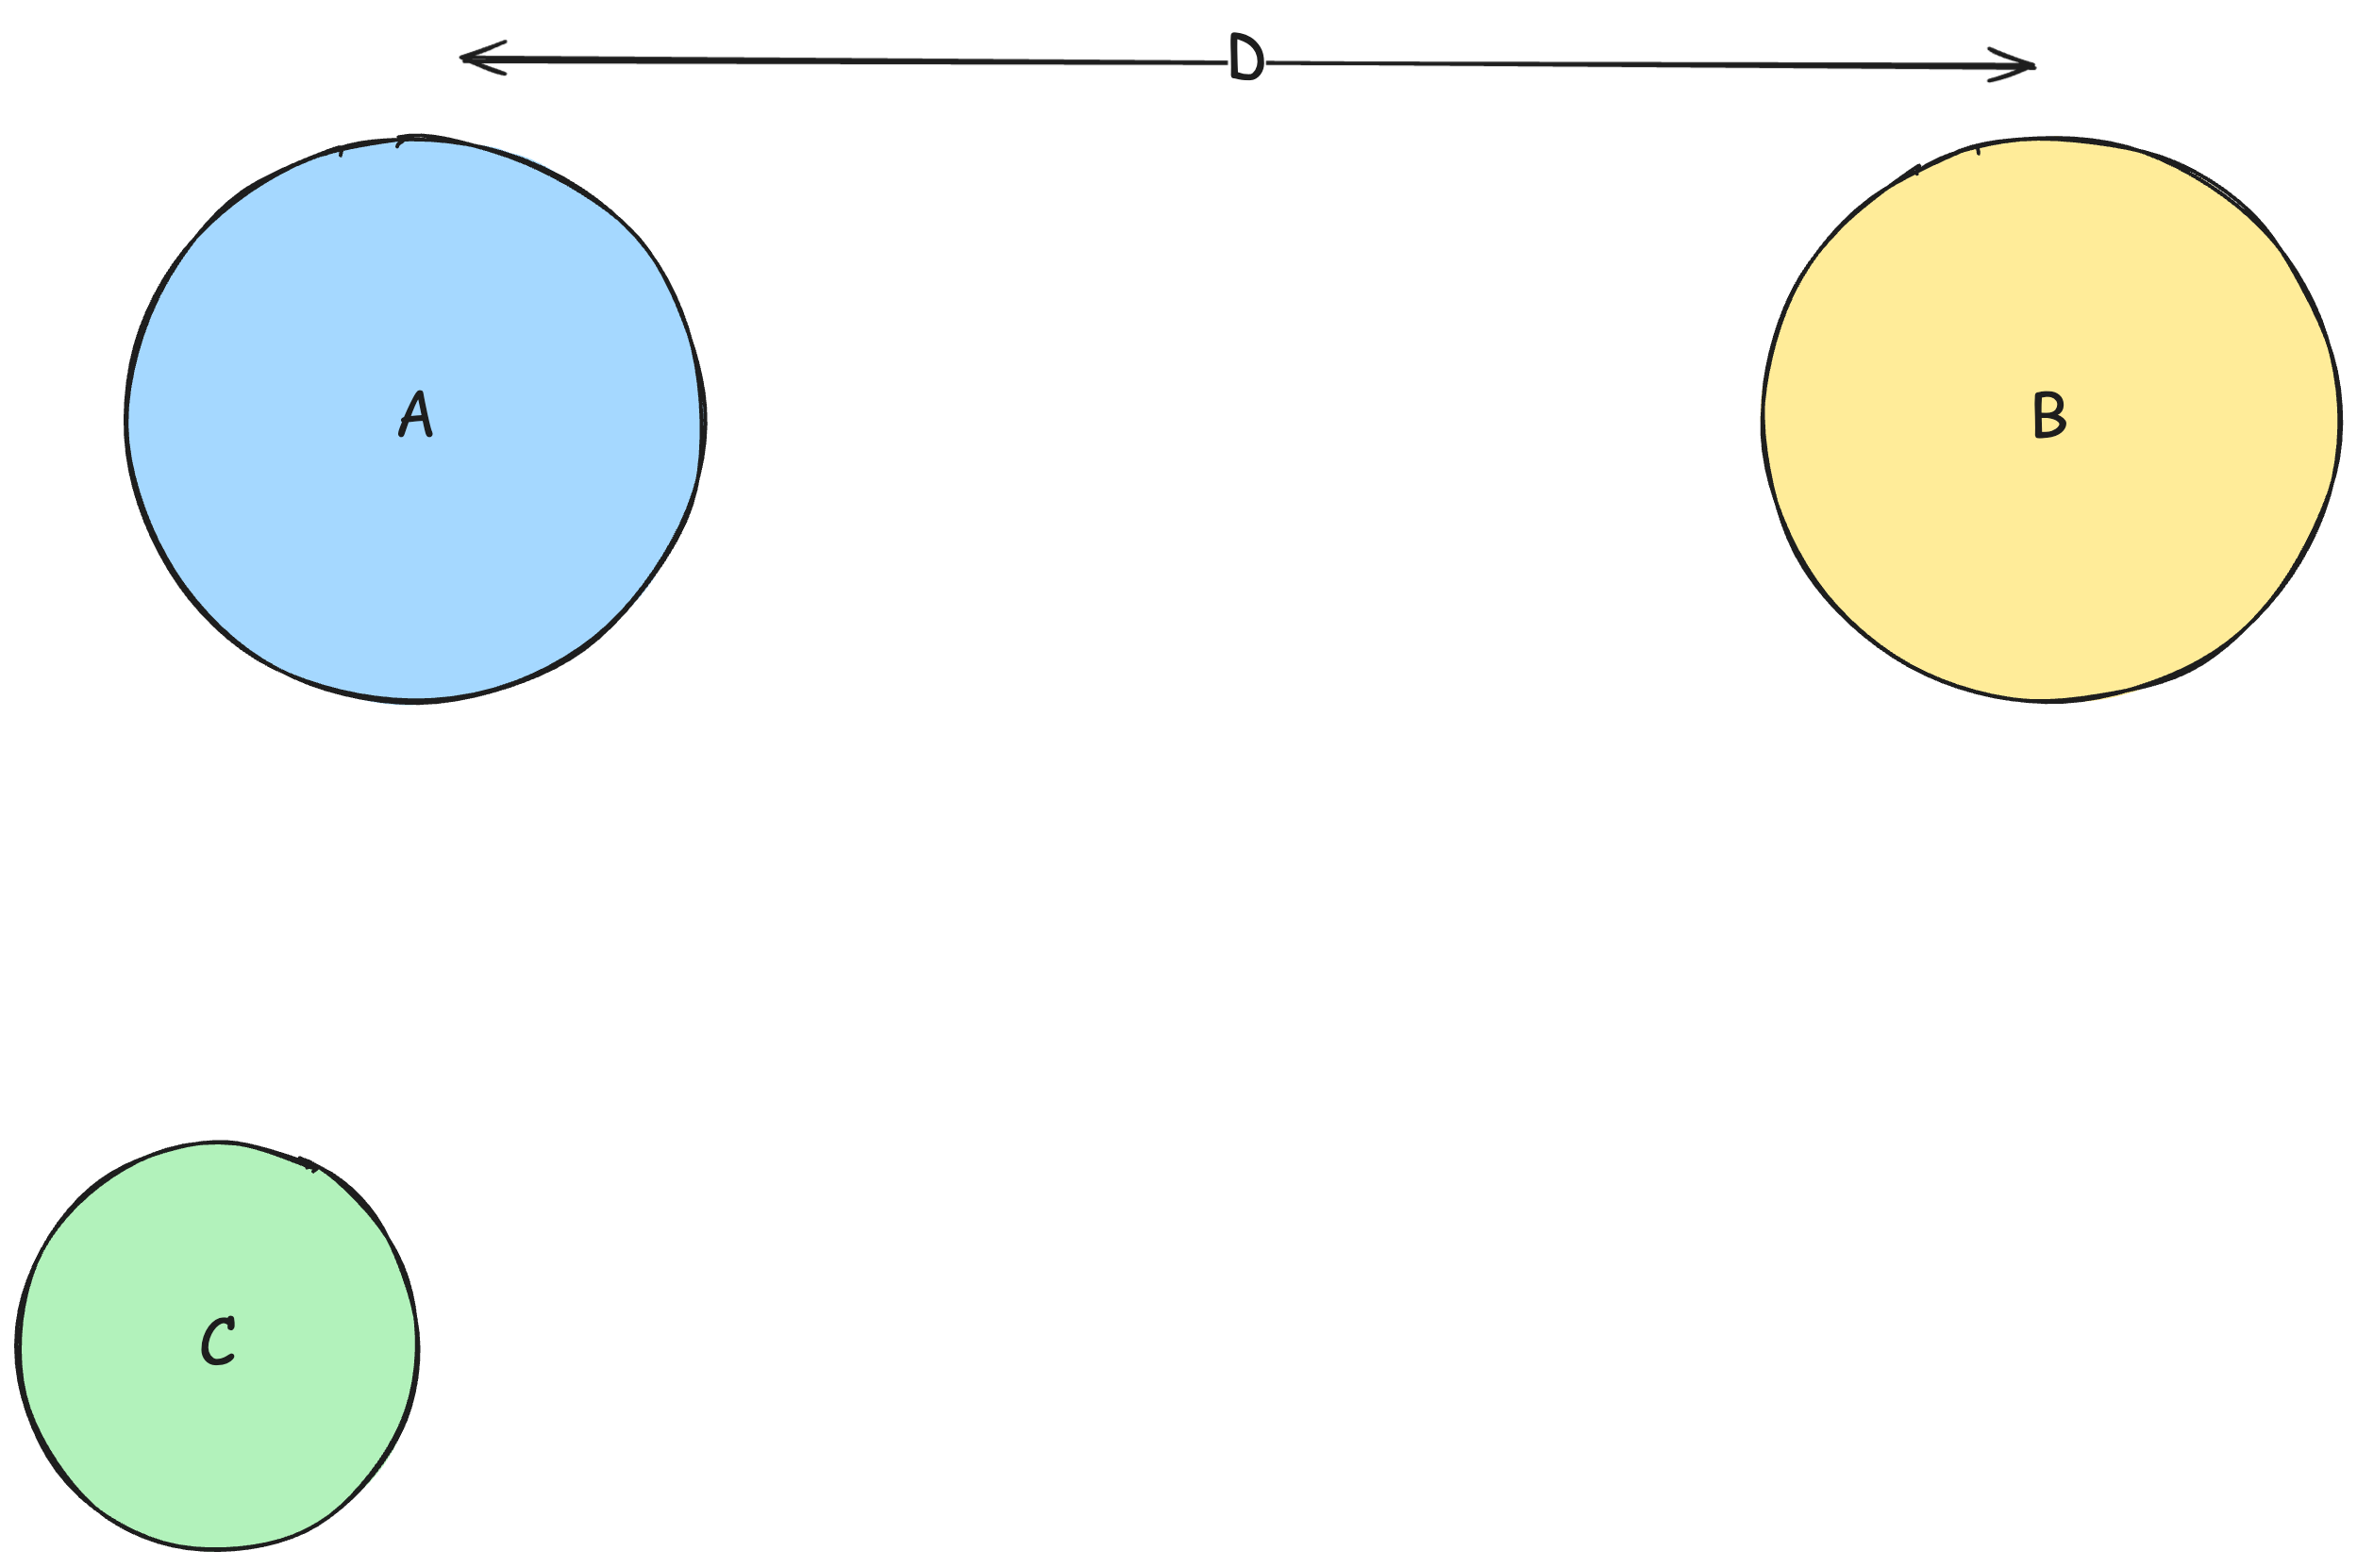
\includegraphics[width=0.2\textwidth]{images/Q8.png}
\end{figure}
To solve this problem, one has to track the changes to the charges over time. Let's do that with a table.
\begin{center}
    \begin{table}[H]
        \caption{Experiment 1}
        \centering
        \begin{tabular}{|c|c|c|c|}
            \hline
            Step & $A_{\text{charge}}$ & $B_{\text{charge}}$ & $C_{\text{charge}}$ \\
            \hline
            0    & 4Q                  & -6Q                 & 0                   \\
            \hline
            1    & 2Q                  & -6Q                 & 2Q                  \\
            \hline
            2    & 2Q                  & -2Q                 & -2Q                 \\
            \hline
        \end{tabular}
    \end{table}
\end{center}


\begin{center}
    \begin{table}[H]
        \caption{Experiment 2}
        \centering
        \begin{tabular}{|c|c|c|c|}
            \hline
            Step & $A_{\text{charge}}$ & $B_{\text{charge}}$ & $C_{\text{charge}}$ \\
            \hline
            0    & 4Q                  & -6Q                 & 0                   \\
            \hline
            1    & 2Q                  & -3Q                 & -3Q                 \\
            \hline
            2    & $-\frac{1}{2}Q$     & -3Q                 & $-\frac{1}{2}$Q     \\
            \hline
        \end{tabular}
    \end{table}

    Given that we know have the tables with the different charges, all is needed is to find the differece in the electrostatic force, and since everything except the charges stays the same, the resolution is simpily a division.
    $$\frac{\frac{-1}{2} \times -3}{2 \times 2} = \frac{3/2}{4} = \boxed{\frac{3}{8}}$$
\end{center}

\section*{13}
\emph{In the figure below, particle 1 of charge $+1.0 \mu \text{C}$ and particle 2 of charge $-3.0 \mu \text{C}$ are held at separation $L = 10 \text{cm}$ on the x axis. If particle 3 of unknown charge q3 is to be located such that the net electrostatic force on it on particles 1 and 2 is zero, what must be the \textbf{(x)} and \textbf{(y)} coordinates particle 3.}
\begin{figure}[H]
    \centering
    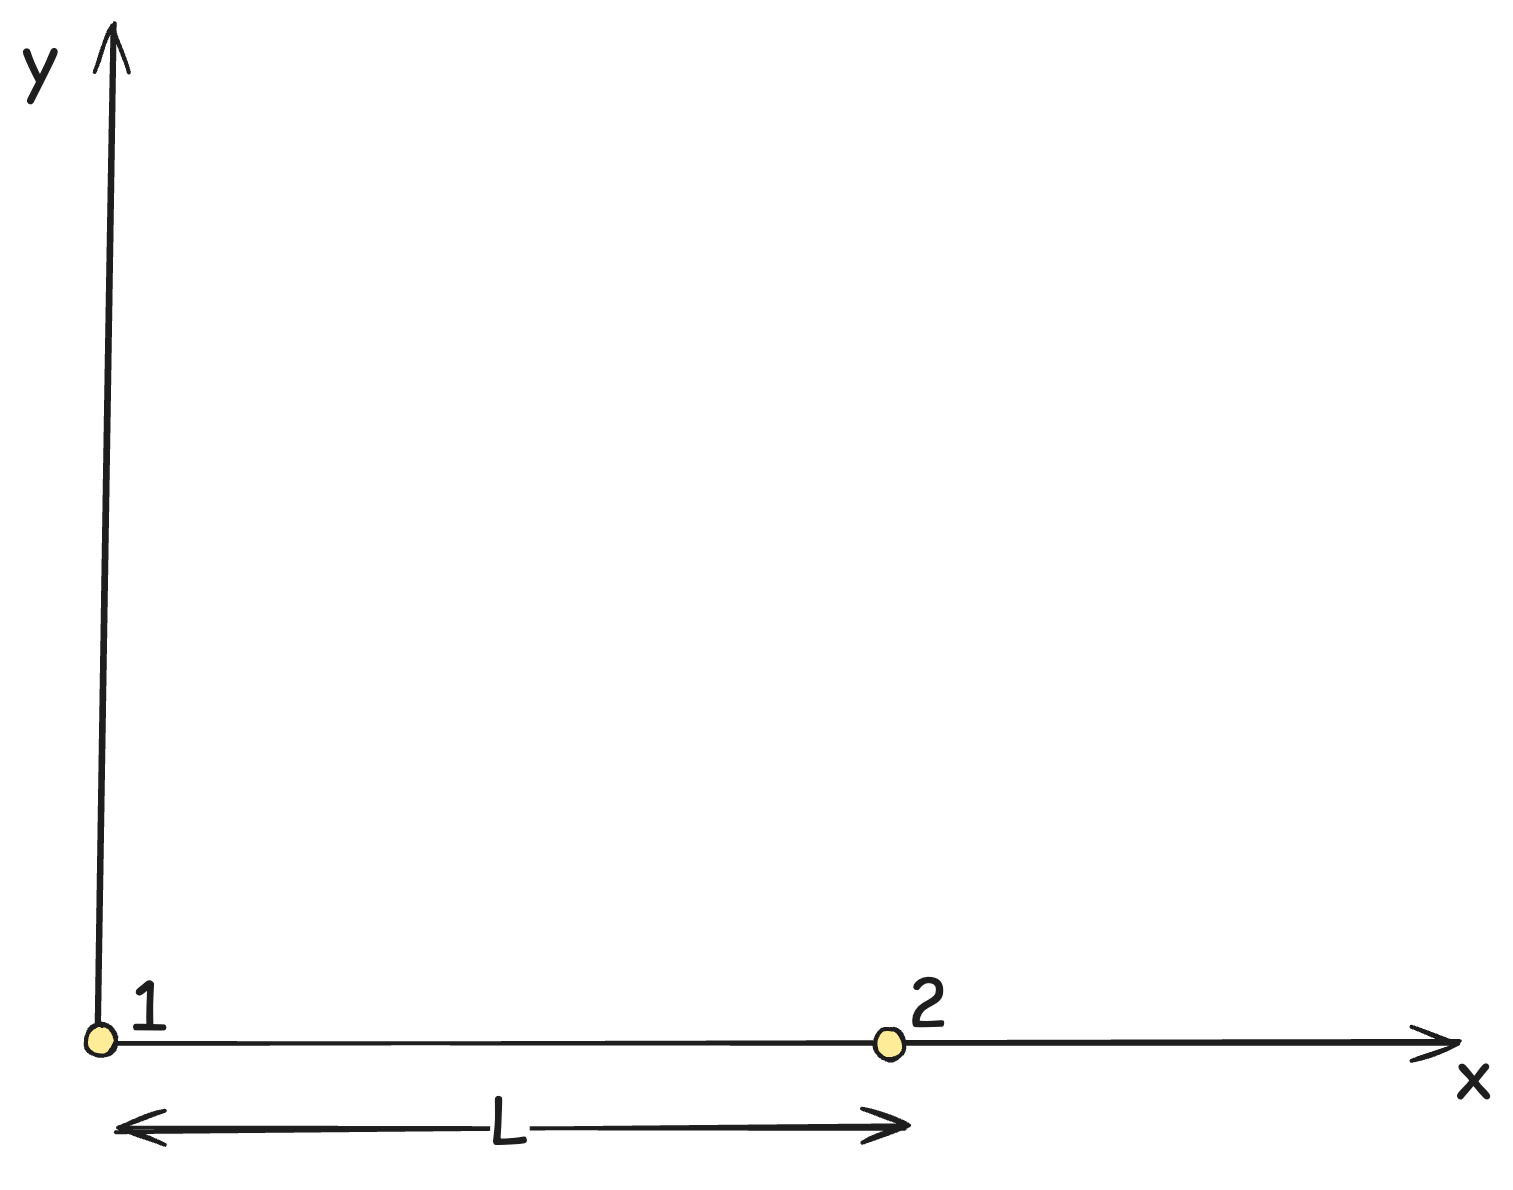
\includegraphics[width=0.4\textwidth]{images/Q13.png}
\end{figure}
Solve using a equality of forces principle. Let's use another image to have the variables make more sense.
\begin{figure}[H]
    \centering
    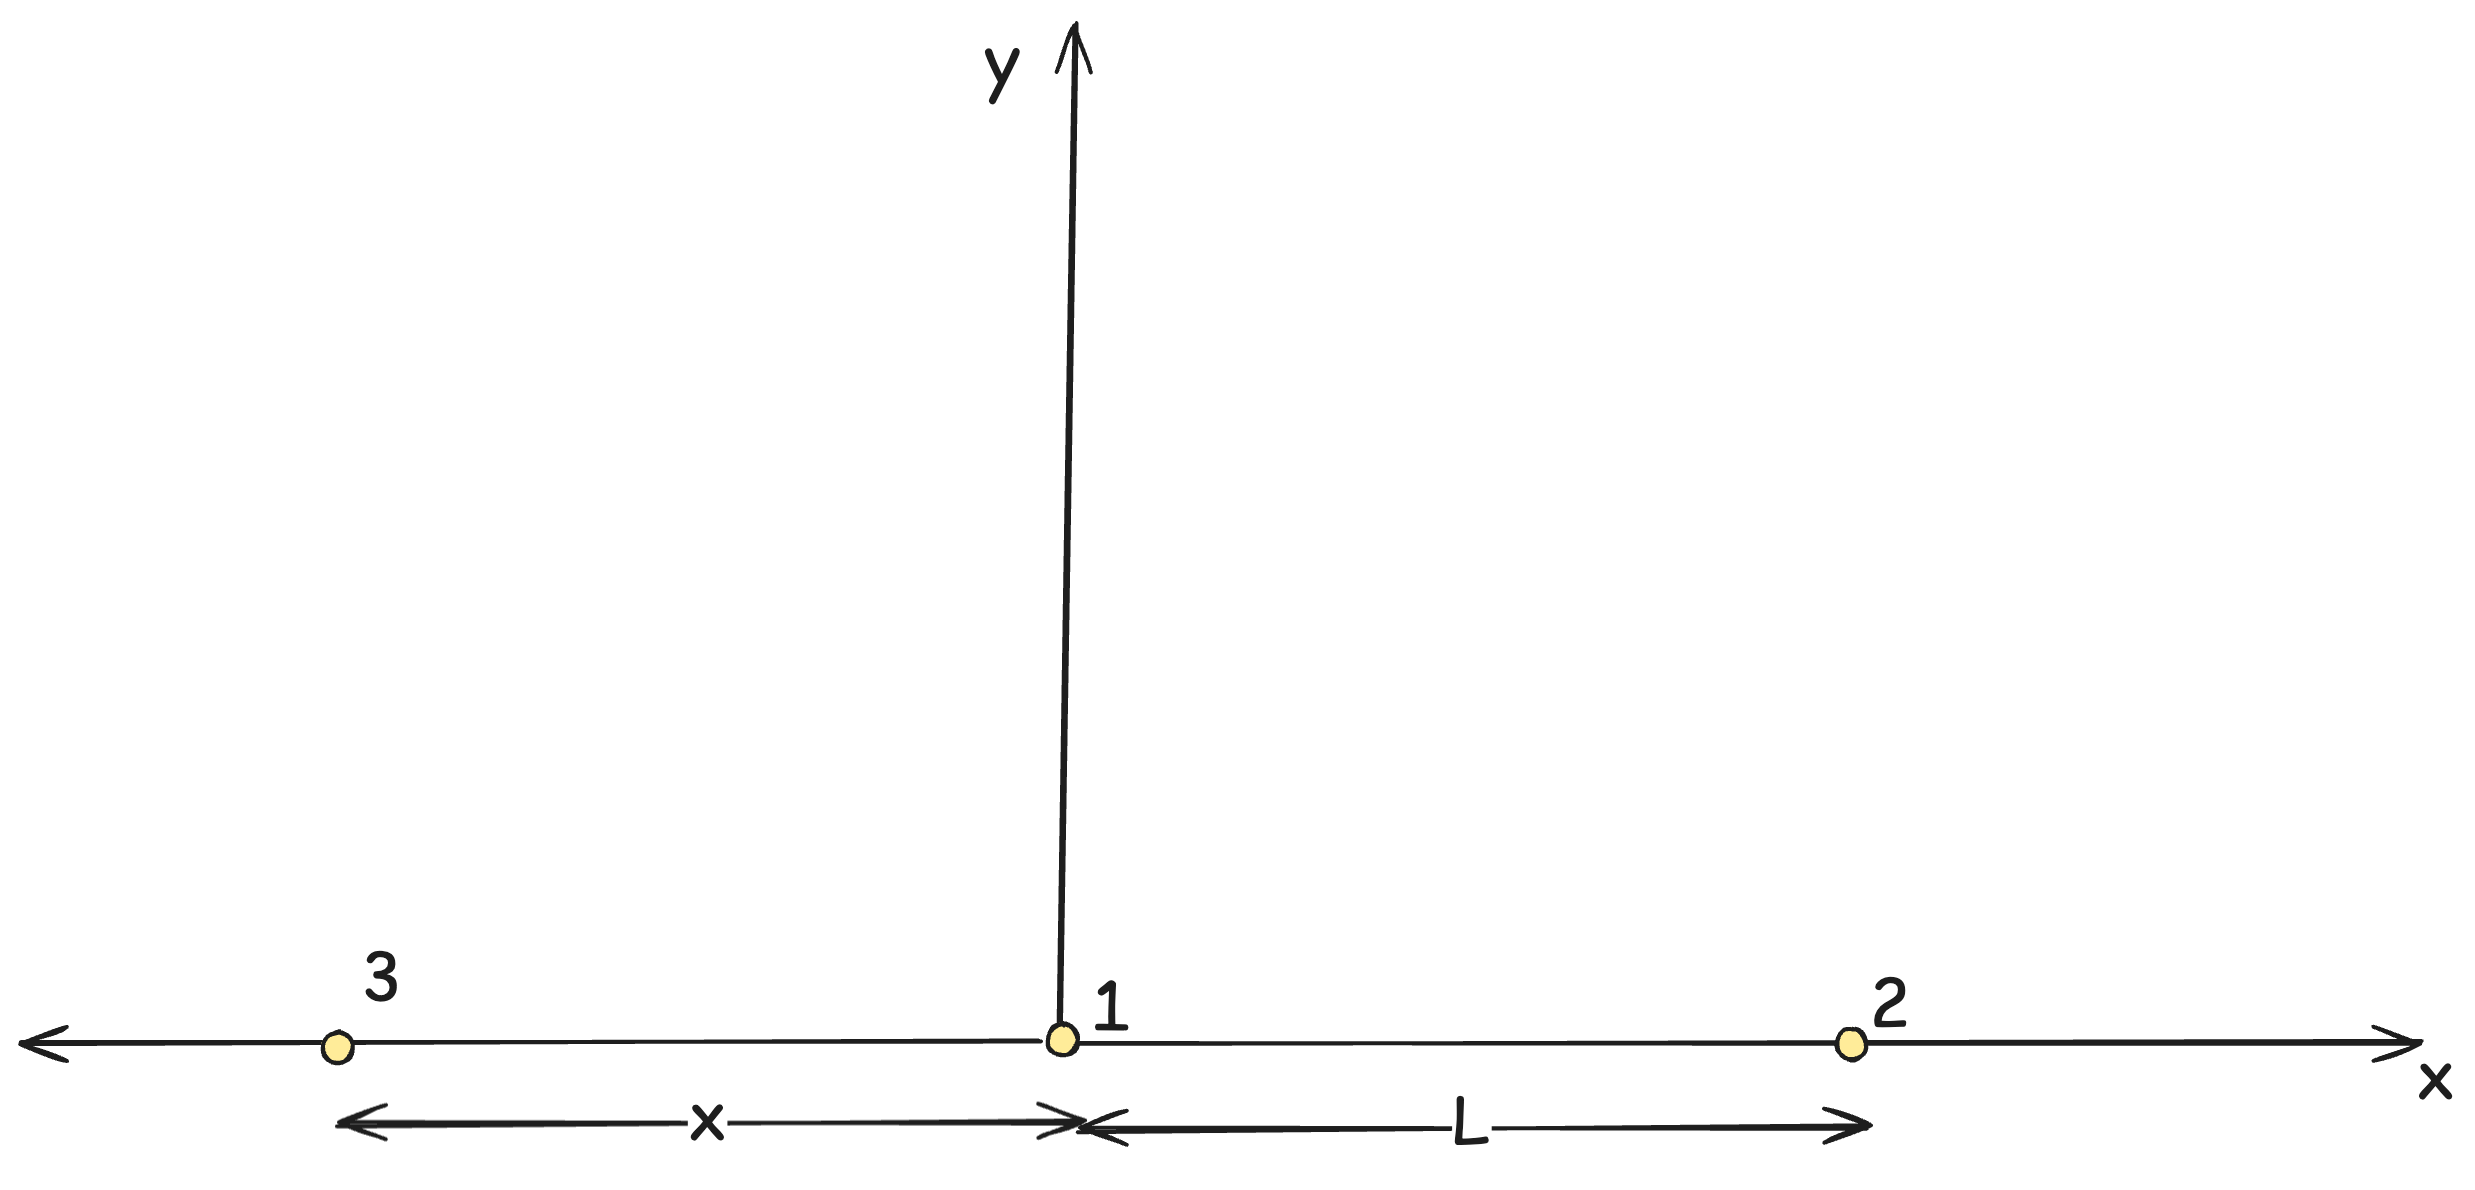
\includegraphics[width=0.6\textwidth]{images/Q13A.png}
\end{figure}
$$F_1 - F_2 = 0 = \frac{1}{4\pi \epsilon} \frac{q q_3}{x^2} - \frac{1}{4 \pi\epsilon} \frac{3q q_3}{(x+.1)^2} $$
$$0 = \frac {q q_3} {x^2} - \frac{3q q_3}{(x+.1)^2} $$
$$-2x^2 + .2x +.01 = 0$$
$$d = \boxed{13.6 \text{ cm}}$$


\section*{19}
\emph{Referring to the figure above (from question 13), particle 1 of charge +q and particle 2 of charge +4.00q are held at separation $L = 9.00 \text{ cm}$ on the x-axis. If particle 3 of charge $q_3$ is to located such that the three particles remain in place when  released, what much be the \textbf{(x)} and \textbf{(y)} coordinates of particle 3, and \textbf{(b)} the ratio $\frac{q_3}{q}$}
To make more sense, let's use this image:
\begin{figure}[H]
    \centering
    \includegraphics[width=0.3\textwidth]{images/Q19.png}
\end{figure}
$$\sum F_1 = \sum F_2 = \sum F_3$$
$$ F_1 = 0 = \frac{1}{4\pi\epsilon}\frac{q_3 q}{x^2} - \frac{1}{4\pi\epsilon}\frac{4q^2}{(0.09 \text{ m})^2}$$
$$0 = \frac{q_3 q}{x^2} - \frac{4q^2}{(0.09 \text{ m})^2}$$

$$F_3 = 0 = \frac{1}{4\pi\epsilon} \frac{q q_3}{x^2} - \frac{1}{4\pi\epsilon} \frac{4q q_3}{(0.09 - x)^2}$$
$$\frac{4}{(0.09 -x) ^2} = \frac{1}{x^2}$$
$$4x^2 = (0.09 - x) ^ 2$$
$$4x^2 = x^2 - 0.018x + 0.0081$$
$$3x^2 + 0.18x - 0.0081 = 0$$
Solve the quadratic using the quadratic formula:
$$\frac{-0.18 + \sqrt{(0.18)^2 - 4(3)(-.0081)}}{2\times3}$$
\textbf{(a)} $\boxed{x = 0.03 \text{ m}}$
\textbf{(b)} $\boxed{y = 0}$

$$q_3 = \frac{x^2 4 }{0.009 \text{ m}}$$
$$\frac{q_3}{q} = \frac{4x^2}{0.09 \text{ m}}$$
\textbf{(c)} $\boxed{\frac{q_3}{q} = \frac{-4}{9}}$ \newline  
\textbf{NOTE}: The negative is inferred because if all positive the outer particles would move apart.

\section*{21}
\emph{A nonconducting sphrical shell, with an inner radius of 4.0 cm and an outer radius of 6.0 cm, has charge spread nonuniformly through its volume between its inner and outer surfaces. The \textbf{volume charge density} p is the charge per unit volume, with the unit coulomb per cubic meter. For this shell $p = \frac{b}{r}$, where r is the distance in meters from the center of the shell and $b = \frac{3.0 \mu \text{C}}{\text{m}^2}$. What is the net charge of the shell?} \\
To solve, imagine an onion (with its shells \st{I'm actually cooked I thought onion rings}), which is how charge is distributed. 
$$Q = \int \delta q = \int p \delta V$$
Since $p = \frac{b}{r}$, we'll have to convert $\delta V \to \delta r$
$$V = \frac{4}{3} \pi r^3$$
$$\frac{\delta V}{\delta r} = 4 \pi r ^2$$
$$\delta V = 4 \pi r ^2 \delta r$$
Let's plug this back into the equation.
$$\int p \delta V = \frac{b}{r} \int 4 \pi r^2 \delta r $$
$$ = 3.0 \frac{\mu \text{C}}{m} \int r \delta r $$
$$ = 3.0 \times 10 ^ {-6} \frac{C}{m} 4\pi \frac{r^2}{2} \big|_{0.04}^{0.06}$$
$$ = \boxed{3.76 \times 10 ^ {-8} C } $$

\section*{32} 
\emph{The figure below shows charged particles 1 and 2 that are fixed in place on an x axis. Particle 1 has a charge with magnitude of $|q_1|=8.00 e$. Particle 3 of charge $q_3 = +8.00e$ is initially on the x axis near particle 2. Then particle 3 is gradually moved in the positive direction of the x axis. As a result, the magniture of the new electrostatic force $F_{2, \text{net}}$ on particle 2 due the particle 1 and 3 changes. The graph gives the x componet of the net force as a function of the position x of particle 3. The scale of the x axis is set by $x_s = 0.80 m$. the plot has an asymptote of $F_{2, \text{net}}$ as $x \to \infty$. As a multiple of e and including the sign, what is the charge $q_2$ of particle 2.} 
\begin{figure}[H]
    \centering
    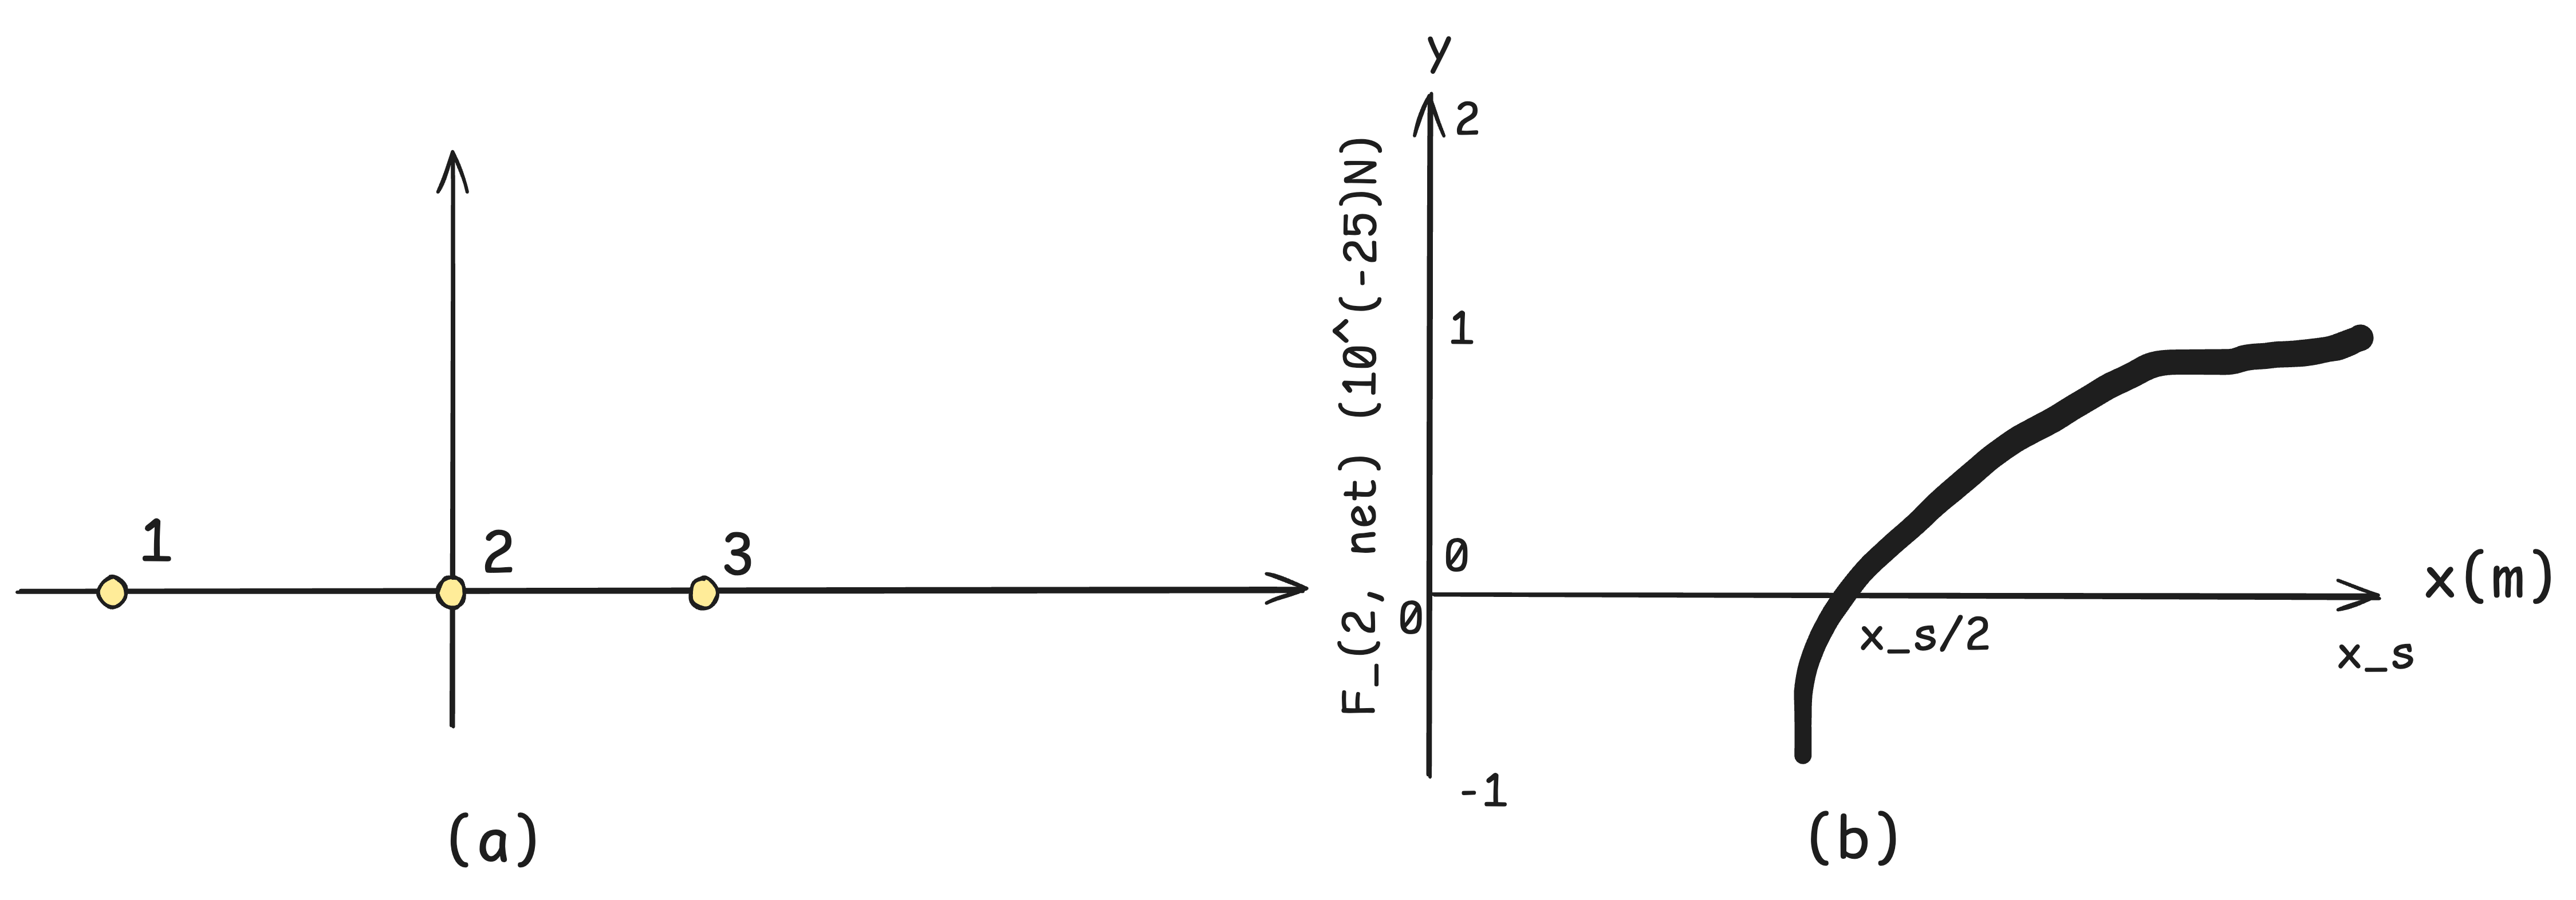
\includegraphics[width=0.9\textwidth]{images/Q32.png}
\end{figure}
Since we know the asymptotic value of the force when the second particle approaches infinity, and an equilbrium (when the net force is zero), we respectively know the force that 1 exerts on two and that the magnitudes of force of $q_1$ and $q_2$ are equal.\\
Let's first start with the $F_{1, 2}$ idea.
$$F_{1,2} = 1.5 \times 10^{-25} N = \frac{1}{4\pi\epsilon_0} \frac{q_1 q_2}{(0.4m)^2}$$\footnote{using $\epsilon_0$ for assumptions sake}
$$q_2 = \frac{1.5\times10^25 N \times 4\pi \epsilon_0 (0.4 m) ^2}{q_1}$$
$$= 2.885 \times 10^{-18} =\boxed{ 13 e}$$. \\
\textbf{NOTE}: We also know the particle is positive because because the force on it is more negative (AWAY from particle 3) the closer the positive particle $q_3$ moves to it. 


\end{document}